The ez\-L\-C\-D modules contains a G\-P\-U an related circutry to drive a L\-C\-D display, U\-S\-B interface \par
 Internal 4mb M\-S\-D flash drive for storage of fonts, bitmaps and macros.\par
 Display can be controlled through U\-S\-B C\-D\-C Serial or T\-T\-L 3.\-3v Serial .\par
 \par
 Once power is applied to the display it starts up and executes startup.\-ezm, it will look in /\-E\-Z\-U\-S\-E\-R/\-M\-A\-C\-R\-O\-S and if not found will look in /\-E\-Z\-S\-Y\-S/\-U\-S\-E\-R\-S .\par
 What this file does in set all defaults for the Display and communcations port.\par
 Including some default widget fonts and themes. \par
 Its best to have a minimal one in the /\-E\-Z\-U\-S\-E\-R/\-M\-A\-C\-R\-O\-S directory with only the relevent settings in it . \par
 \par
 Sample minimal startup.\-ezm. 
\begin{DoxyCodeInclude}
\textcolor{stringliteral}{'minimal startup.ezm}
\textcolor{stringliteral}{}
\textcolor{stringliteral}{'}Turn off \hyperlink{group___general_ga350c2e1be0d3d074d79d7a7278c44a22}{verbose} echo of commands
\hyperlink{group___general_ga350c2e1be0d3d074d79d7a7278c44a22}{verbose} off

\textcolor{stringliteral}{'Set command port to USB CDC}
\textcolor{stringliteral}{cmd cdc}
\textcolor{stringliteral}{}
\textcolor{stringliteral}{'}\textcolor{keyword}{set} some fonts \textcolor{keywordflow}{for} widgets
\hyperlink{group___widgets_ga0efc2d431900e2b77a30e19bb556fb3a}{fontw} 0 0
\hyperlink{group___widgets_ga0efc2d431900e2b77a30e19bb556fb3a}{fontw} 1 0
\hyperlink{group___widgets_ga0efc2d431900e2b77a30e19bb556fb3a}{fontw} 2 0
\hyperlink{group___widgets_ga0efc2d431900e2b77a30e19bb556fb3a}{fontw} 3 serif24
\hyperlink{group___widgets_ga0efc2d431900e2b77a30e19bb556fb3a}{fontw} 4 serif24
\hyperlink{group___widgets_ga0efc2d431900e2b77a30e19bb556fb3a}{fontw} 5 serif24
\hyperlink{group___widgets_ga0efc2d431900e2b77a30e19bb556fb3a}{fontw} 6 serif24
\hyperlink{group___widgets_ga0efc2d431900e2b77a30e19bb556fb3a}{fontw} 7 serif24

\textcolor{stringliteral}{'Set some themes for widgets}
\textcolor{stringliteral}{theme 0   1   2 0 0 0  3  3   1 0 0}
\textcolor{stringliteral}{theme 1 155 152 3 3 3  24  4   5 0 1}
\textcolor{stringliteral}{theme 2   5  20 3 3 3  4  4   5 0 2}
\textcolor{stringliteral}{theme 3   9   3 0 0 0  8  8   9 0 3}
\textcolor{stringliteral}{theme 4   7   3 0 0 0  6  6   6 6 4}
\textcolor{stringliteral}{theme 5 126 118 3 3 3 35 35  36 0 5}
\textcolor{stringliteral}{theme 6 111 106 3 3 3 12 12 101 0 6}
\textcolor{stringliteral}{theme 7  58  48 3 3 3 14 14  54 0 7}
\textcolor{stringliteral}{}
\textcolor{stringliteral}{color white}
\textcolor{stringliteral}{print "Python CDC Mode 115200 Baud  "}
\textcolor{stringliteral}{'}print device model
print 65
print \textcolor{stringliteral}{"  "}
\textcolor{stringliteral}{'print firmware version}
\textcolor{stringliteral}{print 66}
\end{DoxyCodeInclude}
 The ez\-L\-C\-D by default will load startup.\-ezm but you can have startup1.\-ezm through startup5.\-ezm \par
 So if you press the touch screen at power up in any of the areas show below you can execute the other startup macros.\par
  
\begin{DoxyImageNoCaption}
  \mbox{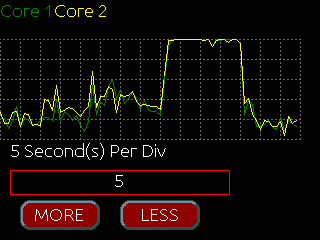
\includegraphics{load.png}}
\end{DoxyImageNoCaption}
